%%%%%%%%%%%%%%%%%%%%%%%%%%%%%%%%%%%%%%%%%
% University/School Laboratory Report
% LaTeX Template
% Version 3.1 (25/3/14)
%
% This template has been downloaded from:
% http://www.LaTeXTemplates.com
%
% Original author:
% Linux and Unix Users Group at Virginia Tech Wiki 
% (https://vtluug.org/wiki/Example_LaTeX_chem_lab_report)
%
% License:
% CC BY-NC-SA 3.0 (http://creativecommons.org/licenses/by-nc-sa/3.0/)
%
%%%%%%%%%%%%%%%%%%%%%%%%%%%%%%%%%%%%%%%%%

%----------------------------------------------------------------------------------------
%	PACKAGES AND DOCUMENT CONFIGURATIONS
%----------------------------------------------------------------------------------------

\documentclass{article}

\usepackage[version=3]{mhchem} % Package for chemical equation typesetting
\usepackage{siunitx} % Provides the \SI{}{} and \si{} command for typesetting SI units
\usepackage{graphicx} % Required for the inclusion of images
\usepackage{natbib} % Required to change bibliography style to
\usepackage{hyperref}
\usepackage{makeidx}

% \setlength\parindent{0pt} % Removes all indentation from paragraphs

\renewcommand{\labelenumi}{\alph{enumi}.} % Make numbering in the enumerate environment by letter rather than number (e.g. section 6)

%\usepackage{times} % Uncomment to use the Times New Roman font

% Para usar el español sin demasiadas complicaciones

\usepackage[spanish]{babel}
\selectlanguage{spanish}
\usepackage[utf8]{inputenc}
%----------------------------------------------------------------------------------------
%	DOCUMENT INFORMATION
%----------------------------------------------------------------------------------------

\title{Analisis y estudio del protocolo Miracast} % Title

\author{Adrian Orduña Diaz, Rafael Leyva Ruiz \\ Grupo 13} % Author name

\date{\today} % Date for the report

\makeindex % Añade un indice al documento

\begin{document}

\maketitle % Insert the title, author and date

\tableofcontents

% If you wish to include an abstract, uncomment the lines below
% \begin{abstract}
% Abstract text
% \end{abstract}

%----------------------------------------------------------------------------------------
%	Introduccion
%----------------------------------------------------------------------------------------

\section{Introducción}

Miracast es definido en la web de \href{http://www.wi-fi.org/discover-wi-fi/wi-fi-certified-miracast}{WiFi Alliance} más como una certificación más que como un protocolo, ya que para su funcionamiento se basa en diversos protocolos que trabajan todos juntos, pero igualmente se puede analizar desde el punto de vista de considerarlo un protocolo en sí, debido a la gran cantidad de requerimientos técnicos que conlleva y su forma de trabajar, que propiamente define un protocolo de conexión, aunque el, llamemoslo asi, trabajo sucio lo realizan otros protocolos. Por eso este documento busca dar una introducción y base de conocimientos acerca de Miracast, su funcionamiento desde un punto de vista técnico, utilidades y beneficios a nivel de usuario.


\section{Historia}

Miracast fue anunciado en 2013 en el congreso tecnologico de las vegas conocido como CES por la Wifi Alliance, era un protocolo revolucionario que permitia compartir contenidos multimedia inalambricamente, al igual que hasta el momento se podía hacer con un cable hdmi o VGA con la inestimable ventaja de poder prescindir de los cables, ya que todo funciona inalambricamente.
\\
La certificacion miracast tuvo un gran calado en la industria de consumo multimédia, y en pocos meses todos los grandes de la electronica de consumo anunciaron nuevos productos compatibles con esta tecnología, como televisiones, moviles, etc.
\\
Aunque no seria hasta octubre del año siguiente y los meses que lo seguirían que esta tecnología viviría su mayor empuja, gracias a la competencia Apple vs Google. La primera había anunciado Airplay, un estandar similar a miracast, y Google en su intento por no quedar atras en esa carrera tecnológica añadio miracast al código fuente de android, facilitando asi que todos los fabricantes de su ecosistema pudiesen implementar facilmente esta tecnología, con lo que se produjo una gran expansión de dispositivos compatibles.
\\
El segundo gran empujon llego con la presentación de chromecast, un dongle HDMI que conectandose al puerto HDMI de una pantalla y compartiendo el mismo wifi que un pc o un movil, era capaz de hacer mirroring en la pantalla, con las grandes aplicaciones que esto presenta.
\\
A dia de hoy una gran cantidad de disposítivos y aplicaciones hacen uso de Miracast para ampliar su utilidad y seguir facilitando la vida a los usuarios.


\section{Usos y aplicaciones}

Ya se han ejemplificado varios escenarios en los que la tecnología Miracast puede resultar muy práctica. Siendo muy usada por ejemplo para mostrar datos y presentaciones en reuniones empresariales, ya que permite conectar el pc a un proyector compatible en pocos segundos y empezar, sin cables de por medio. También es muy usado en el ámbito informático, ya que gracias al mirroring se pueden mostrar demos muy fácilmente en cualquier momento.

En el ámbito doméstico, da facilidades para compartir contenido con un gran número de personas mediante una televisión compatible, como mostrar las fotos de las vacaciones en la tele, reproducir música por los altavoces de una fiesta, o incluse realizar videollamadas haciendo uso de la televisión, aunque todo esto requiere tener el dispositivo emisor siempre encendido.

Por otro lado la tecnología que usa por debajo, WiFi Direct es muy usada para intercambio de archivos, se habla de que incluso podría reemplazar al Bluetooht, ya que puede conectar a varios dispositivos en una LAN sin necesidad de router, y gracias a su funcionamiento P2P el crecimiento que podría experimentar esta LAN es enorme, ya que los nuevos dispositivos se conectan a otros que ya hay conectados, no al que se estableció como punto de acceso original.

Todo esto se vera con más detalle cuando estudiemos los apartados técnicos del protocolo.


\section{¿Qué es?}

Miracast es una nueva tecnología que quiere acabar con los HDMI y evitar el uso excesivo de cables.

Miracast es un nuevo estándar para la transmisión de audio, imagen y video mediante WiFi. Gracias a ésto, podremos disfrutar de cualquier contenido multimedia en cualquier aparato de nuestro entorno.  Miracast se basa en el "screen mirroring" de Android.  El protocolo está basada en WiFi Direct, es decir, permitir que varios dispositivos se conecten entre sí, sin necesidad de un punto de acceso intermedio. Esta tecnología te permite transmitir y visualizar el contenido multimedia que desees de forma individual o simúltanea entre varios dispositivos.




\section{¿Cómo funciona?}

El funcionamiento de Miracast es sencillo, conectar todos los dispositivos sin necesidad de Internet, solo necesitan estar conectados a una red local. Tanto el dispositvo emisor como el receptor deben soportar la tecnología Miracast para funcionar. Sin embargo, para transmitir contenido multimedia a un dispositivo que no es compatible con Miracast, existen adaptadores que se conectan a los puertos HDMI o USB.

Miracast permite a un dispositivo portátil, ya sea móvil o tablet, o a un ordenador enviar, de forma segura, vídeo de alta definición hasta 1080p y sonido envolvente 5.1. Permite a los usuarios, por ejemplo, duplicar la pantalla de sus smartphones en un televisor, e incluso compartir la pantalla de un ordenador portátil con el proyector en una sala de coferencias en tiempo real, para que todos los asistentes puedan ver, por ejemplo una presentación.


%----------------------------------------------------------------------------------------
%      Apartado tecnico
%----------------------------------------------------------------------------------------

\section{Proceso de conexion de dispositivos mediante miracast}

Como hemos contado anteriormente el protocolo miracast facilita mucho el proceso de conexión de dispositivos con el objetivo de compartir contenido multimedia, pero como se ejecuta este proceso internamente, ya que el usuario solo pulsa un boton en su dispositivo y la conexion es automática.

\subsection{Identificación de dispositivos}

Cuando se intentan parear dos dispositivos para que sean usados con el protocolo miracast 1 de los dispositivos, el que realizara el envio de contenido normalemte, se establece como el primer host de una red WiFi Direct, redes preparadas para el intercambio de ficheros mediante P2P de las que hablaremos mas adelante, y el segundo escanea los dispositivos que hay con esta condición en su rango de alcance. Tras esto se envia una peticion de conexión mediante WPS al dispositivo que hace como localHost primario en la LAN WiFi Direct.

\subsection{Verificación de la conexión}

Una vez que el localHost recive la petición de conexion mediante WPS normalmente pedirá confirmacion, tras la cual dara permiso al segundo dispositivo para entrar a formar parte de la red local formada, en esta primera instancia por dichos dos dispositivos, aunque se podrían ir incorporando mas dispositivos, y se inicia la transferencia de archivos.

\subsection{Transferencia de datos}

Los datos se transmiten, en un principio, en un solo sentido, lo cual indica que no se tiene un feedback de que esta pasando cuando los datos llegan al receptor. Esto se realiza mediante la red WiFi Direct gracias o bien al protocolo RTSP o bien RTP, los cuales poseen conexión cifrada y presentan una gran seguridad para evitar el posible robo de información mediante el intercambio. El receptor simplemente se dedica a recoger los datos y gestionarlos debidamente.

En posteriores actualizaciones, o enmascarando el protocolo en una capa superior se podria dotar de la funcionalidad de feedback por parte del receptor, lo cual en diversos escenarios como streamings de grandes cantidades de datos podrian ser útiles, por ejemplo para dejar de ocupar la banda ancha.


\section{WiFi Direct}

La definición de WiFi Direct por la WiFi Alliance, organización creadora de esta tecnología, como una \"certificación para diferentes dispositivos que soportan cierta tecnología que permite la comunicación directa\", en otras palabras, permite conectar distintos dispositivos sin necesidad de cables. Esta tecnología es en la que se basa el protocolo Miracast.

WiFi Direct es en esencia un punto se acceso en forma de software, los llamados \'Soft AP\'. El Soft AP proporciona una versión de Wi-Fi Protected Setup o \'WPS\'. Respecto a la seguridad, Wi-Fi Direct incluye seguridad WPA2 y ofrece controlar el acceso a redes corporativas. Los dispositivos certificados para Wi-Fi Direct se pueden conectar \"uno a uno\" o \"uno a muchos\", y no todos estos dispositivos conectados necesitan tener Wi-Fi Direct, con solo un dispositivo Wi-Fi Direct habilitado se pueden conectar los demás dispositivos con el estándar previo de Wi-Fi. Esta tecnología se puede ver claramente, por ejemplo, cuando se comparte internet con otro teléfono móvil.

El funcionamiento de WiFi Direct es similar al de Bluetooth. Un dispositivo con  WiFi Direct activado emite una señal hacia otros dispositivos haciendo saber que está disponible para una conexión. Los usuarios pueden enviar una petición, o recibir una, para efectuar dicha conexión. Cuando ambos o más dispositivos están conectados se puede empezar a compartir archivos.

La principal diferencia con Bluetooth es la mayor tasa de transferencia de archivos, 250Mbps de WiFi Direct respecto a los 25Mbps de Bluetooth 4.0, aunque los dos hagan uso del protocolo 802.11.

En definitiva, Wi-Fi Direct, es una versión actualizada y mejorada de Bluetooth sin necesidad de tener que establecer conexión a Internet.
 %descripcion acerca del protocolo wifidirect

\section{Seguridad}

Respecto a la seguridad, Miracast cuenta con el protocolo de seguridad WPA2.

WPA2 es el nuevo estándar del IEEE (Institute of Electrical and Electronics Engineers) para proporcionar seguridad en redes WLAN. WPA2 incluye el algoritmo de cifrado AES, desarrollado por el NIST (National Institute of Standards and Technology). Se trata de un algoritmo de cifrado en bloque con claves de 128 bits.

WPA2-PSK soporta una contraseña de hasta 63 caracteres alfanúmericos, es decir que la contraseña puede llegar a tener hasta 63 mayúsculas, minúsculas, símbolos y números, por lo que la clave se hace robusta para su descifrado. Además, a partir de la Pre-Shared Key, el sistema va generando nuevas claves que transmite al resto de equipos, lo cual dificulta notablemente la acción de descifrado. Un incoveniente importante es que todos los dispositivos no soportan el modo WPA2-PSK.

En definitiva, respecto a seguridad Miracast cuenta con un gran sistema de protección que dificultad bastante que personas ajenas puedan llegar a visualizar lo que estamos compartiendo a través de este sistema.
 % seguridad en miracast

%\section{CODECs}

Miracast dispone de un códec obligatorio y dos opcionales.

El códec obligatorio es LPCM, 16 bits 48 KHz en 2 canales. LPCM son las siglas de Linear Pulse Code Modulation, es un formato de audio sin compresión que puede llegar a tener hasta 8 canales de audio en una frecuencia que va desde los 48 KHz hasta los 96 KHz. Es muy usado en comunicaciones y ahora también ha sido adoptado por la industria musical. El formato simultáneamente captura y muestrea señales analógicas y las transforma en señales digitales. El PCM Lineal, conocido así en España, fue definido como parte del estándar DVD.

En los códecs opcionales tenemos, AAC (del inglés Advanced Audio Coding) es un formato de señal digital de audio basado en un algoritmo de compresión con pérdida, un proceso por el que se eliminan algunos datos de audio para poder obtener el mayor grado de compresión posible, resultando en un archivo de salida que suena lo más parecido posible al original, éste algoritmo de codificación de banda ancha de audio tiene un rendimiento superior al del MP3, mejor calidad en archivos más pequeños y requiere menos recursos del sistema para codificar y decodificar. El formato AAC corresponde al estándar internacional "ISO/IEC 13818-7" como una extensión de MPEG-2 (Moving Picture Experts Group). Este formato ha sido elegido por Apple como formato principal para los iPods y para su software iTunes. Entre las extensiones de archivo de este formato cabe destacar .m4a, .3gp, .mp4, entre otras.

Por último tenemos el códec AC-3, conocido como Dolby Digital. Es una serie de tecnologías de compresión de audio desarrollado por los laboratorios Dolby. El AC-3 es uno de los formatos denominados de compresión perceptual. Lo que hace, básicamente, es eliminar todas las partes del sonido original, codificado analógicamente, que no pueda ser percibido por el oído humano. De ésta forma, se logra que la misma información sea de menor tamaño y por lo tanto ocupe mucho menos espacio físico. AC-3, es la versión más común que contiene hasta un total de 6 canales de audio, con 5 canales de ancho de banda completo de 20 Hz - 24 KHz para los altavoces de rango normal y un canal de salida exclusivo para los sonidos de baja frecuencia conocida como Low Frequency Effect, o subwoofer. También soporta el uso de Mono y Stereo.
 % codecs multimedia y su soporte en miracast

\section{Protección de contenido con derechos de autor en Miracast}

Con el claro objetivo de ser un cable HDMI pero sin el cable, Miracast provee una interfaz con la cual permite abstraerse completamente sobre los codecs usados por los distintos dispositivos, pero esto plantea la duda acerca de cómo se gestionan los contenidos con copiright. Para ello Miracast provee su propio DRM (Digital Rights Management), el cual emula el sistema usado por los dispositivos HDMI, para dicho propósito usa HDCP, especificación propietaria y desarrollada por Intel con dicho cometido.

Para ello y por requerimiendo de DHCP, si el dispositivo emisor comunica que se van a enviar contenidos protegidos el receptor debe tener implementado su propio gestor de DHCP, que al haber sido licenciado garantiza que el dispositivo receptor debe de frustar los intentos de copia, para así evitar que el contenido sea distribuido libremente o copiado sin previa autorización.

Así si el dispositivo receptor no cumple con esta especificación solo recibe una señal peor de la real, con esto se busca evitar precisamente esa violación de los contenidos con derechos de autor.

Miracast requiere dependiendo de su versión del uso de DHCP en la version 2.1 o 2.2 de dicha especificación, cuyo funcionamiento en dispositivos que esten retransmitiendo por medio de Miracast es el siguiente:

\subsection{Gestión de DHCP en el servidor de contenidos Miracast}

El servidor, de ahora en adelante el dispositivo que emite contenido mediante Miracast, comprueba periódicamente si ha de enviar contenido protegido, si esta comprobación es afirmativa se envian una serie de bits cifrados durante la transmisión que solo si el receptor es capaz de decodificar (lo que indica que cumple con la especificación de DHCP) serán gestionables y además se enviará un feedback al emisor para confirmar la recepcion y correcta gestión de dichos datos. Como se muestra en la figura siguiente, ésto se lleva a cabo en la capa de TCP de transmisión de datos, mediante una conexión con la implementacion de DHCP del dispositivo emisor:

\begin{figure}[ht]
  \begin{centering}
    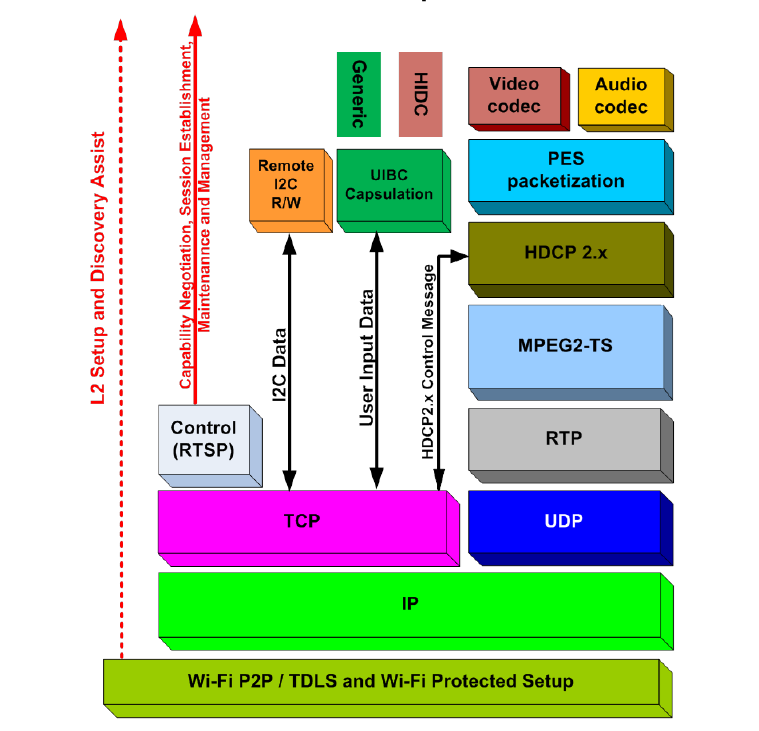
\includegraphics[width=1.0\textwidth]{./Imagenes/HDCP_miracast_layers.png}
    \caption{Ilustración acerca de dónde se ubica HDCP en el protocolo de conexión Miracast}
  \end{centering}
\end{figure}

El receptor simplemente hace la comprobación y gestiona los datos devolviendo un feedback al emisor, por lo que todo el coste de la gestión de DRM recae sobre él.
 % Proteccion del contenido con derechos de autor

%\input{Ejemplo de uso y capturas de whireshark}

%\input{sections/conclusion}
\end{document}
